\newpage
\section{Aire Guru}

Urban residents are surrounded by many sources of air pollution, and it is the direct cause of many different symptoms,
ranging from simple eye irritation 
to, in extreme cases, death. Particularly for high-risk groups like children and the elderly.
The WHO (World Health Organization) estimates 4.2 million deaths
(https://www.who.int/airpollution/ambient/en/) per year due to air pollution.
Air pollution has a significant affect on people with asthma, cardiopathies, allergies, and neurological pathologies.

Air pollution not only aggravates existing diseases, but can also be an initial cause of them, such as in the case of foetal brain
damage (https://www.cronicabalear.es/2018/07/la-contaminacion-ambiental-causa-enfermedades-neurologicas-y-envejecimiento-del-cerebro)
caused by the mother's exposure to air pollution.

To be able to control the level of exposure we need to know the levels
in the specific locations that we frequent, and the variation during specific times.
To make this information as accessible as possible, it should be freely and publicly available, and the presentation
must be simple enough to be understandable by the average citizen.

We have created a tool - Aire Guru - which collects air pollution data periodically, stores it for historical use, 
processes it to extract relevant information, personalizes it to engage the user with regard to their individual
circumstance, visualizes it in an easy to understand format, and provides it online to facilitate its accessibility. Furthermore,
descriptions of all the data and how it has been processed are also provided to raise public awareness of the value
of this data. Aire Guru has been successfully tested, using the Air Quality data provided
by the Málaga open data portal(https://datosabiertos.malaga.eu/) in the Spanish city of Málaga.

There are already many tools available, however they have various failings.

The most common problems are:

\begin{itemize}

\item Obsolete measurements. Measurements need to be taken regularly, since there can be huge differences
between pollution levels at different times of the day.

\item Limited geographic coverage. The data must cover a reasonable proportion of areas that people spend significant time in.

\item Insufficiently granular measurements. Measurements must be at a reasonably fine level of granularity. One single measurement for an entire city is not useful.

\item Poor presentation. Often the information is presented in an uninterpreted form, making it difficult for users to visualize, especially in a geographic sense.

\item Poor discrimination and interpretation. Many tools show individual values as a number or a colour. This information is not
enough for the user to take control of their exposure. Such visualizations are not really compelling. 

\end{itemize}

Our webtool (https://airquality.guru/), solves the deficiencies described above.

Measurements are published hourly and come from measurement stations placed throughout the 
city of Málaga, covering entire urban region at a granularity of $100m^2$

The information is presented in a clear and simple manner, making it possible to see the most polluted regions,
and allowing the user to make comparisons both geographically and historically. It provides personalised information, such as the most relevant 
pollutants for a user's particular medical conditions, and can track
the pollution they are exposed to both in real time and over a historical period, by linking with location data from their mobile device. 

The system has been successfully tested with 14 subject in the Spanish city of Málaga. The survey showed a high degree of satisfaction, 
particularly regarding the clarity and completeness of the the information and analysis.
More than the half of the subjects were not aware of how air quality is measured and how it 
can affect their health. Four of the subjects discovered that they have a medical 
condition which can be affected by air pollution.
    
Aire Guru is available online, free of charge.

\subsection*{Cleaned}

THIS SHOULD BE INCORPORATED INTO A DESCRIPTION OF AIRE GURU

The platforms provide a huge volume of data, since, as mentioned earlier, they collect as much data as possible.
There will be multiple samples containing the specified set of fields. These field sets may be similar to each other but don't need to be identical.
From this data, we need to select the relevant samples, and from these, the fields necessary to represent specific information.

Below we can see examples. The first one is taken from the European open data portal
(https://www.eea.europa.eu/data-and-maps/data/air-pollutant-concentrations-at-station/air-pollutant-concentrations-201) and the second from the North American open data portal
(https://data.cityofnewyork.us/api/views/kku6-nxdu/rows.json?accessType=DOWNLOAD).

\begin{figure}[ht]
    \centering
    \subfigure[EEUU Open Portal. Demographic Statistics By Zip Code]
     {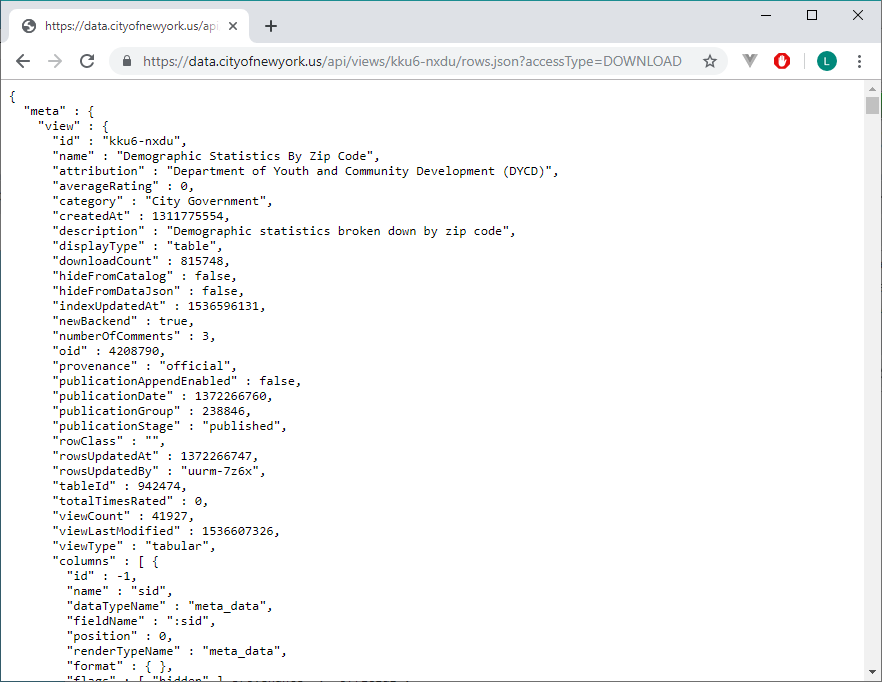
\includegraphics[width=5cm]{ExampleOpenDataEEUU}}
    \hfill
     \subfigure[European Open Data Portal. Air pollutant concentrations 2015]
    {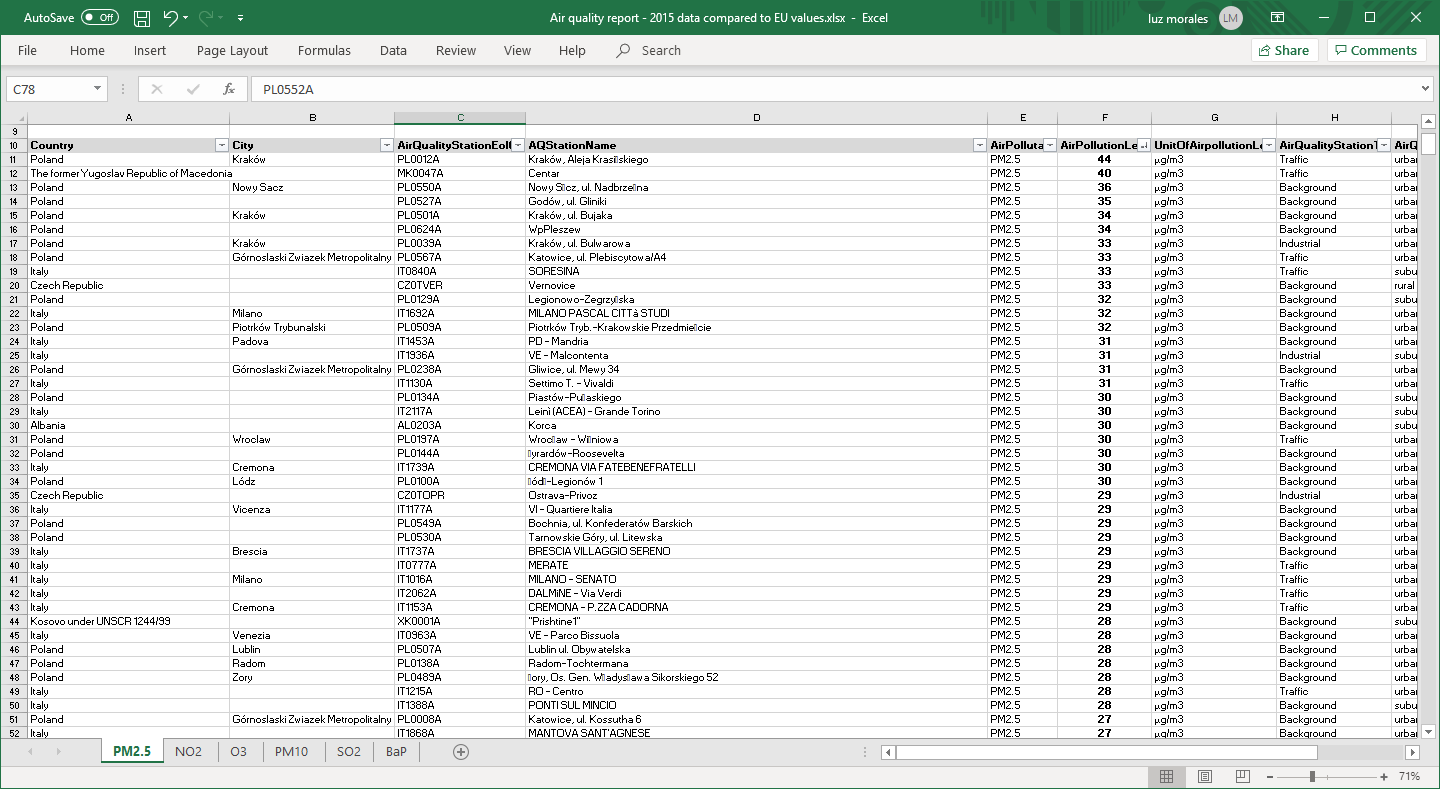
\includegraphics[width=7cm]{ExampleOpenDataEuropean}}
    \caption{Open Data Examples}
\end{figure}
    
\subsubsection*{Suggested strategies}

We obtain our required data through a series of processes such as extraction, transformation and
cleaning of the data. Without automation, these processes are tedious and time consuming. 

\subsubsection*{In the context of Aire Guru \ldots} 

The extracted data is in GeoJSON format, a format which provides a JSON object with nested subdocuments. Each of these
subdocuments contains a set of data in key-value form.
In the following figure we can see the beginning of the document downloaded on June 9, 2019
(https://datosabiertos.malaga.eu/recursos/ambiente/calidadaire/calidadaire.json) \\

\begin{figure}[ht]
    \centering
   \subfigure[First subdocument]{ \centering 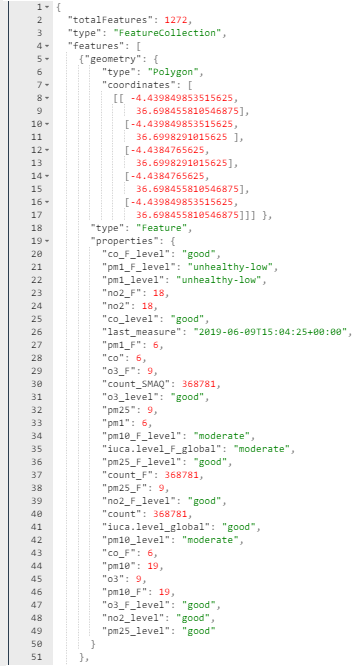
\includegraphics[width=4.75cm]{geoJsonAirQualityData1}}
   \hfill
   \subfigure[Second subdocument]{ \centering 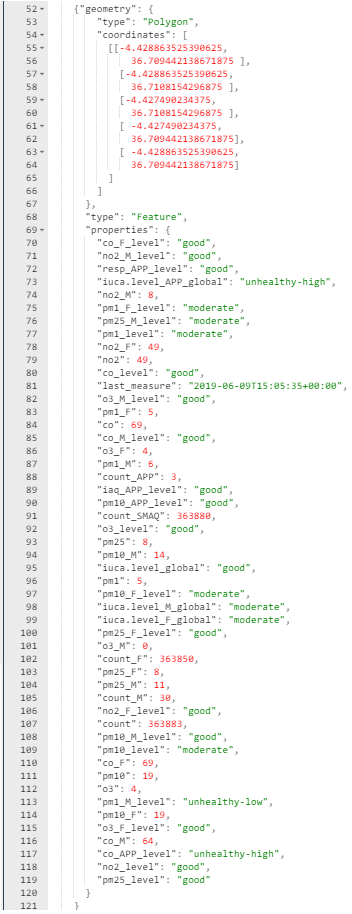
\includegraphics[width=4.75cm]{geoJsonAirQualityData2}}
 
    \caption{Air quality Document [09/06/2019]. Open Data Portal Málaga}
    \end{figure}
    
    In this excerpt we can see the first two subdocuments. Each subdocument contains the coordinates of the air quality 
    measuring station, the date and time when the measurement was recorded, and the values of the measurements.
    In the following figure we can find the description provided by the open data portal.
    
\begin{figure}[ht]
    \centering
    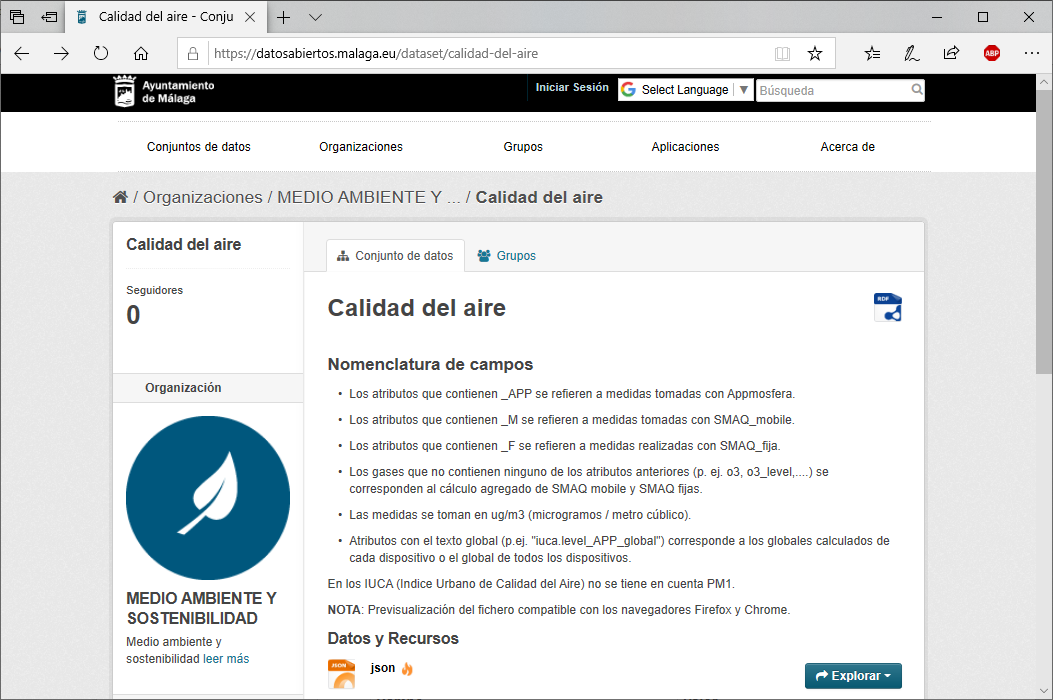
\includegraphics[width=8cm]{geoJsonAirQualityDataDescription}
    \caption{Air quality data description [09/06/2019]. Open Data Portal Málaga}
\end{figure}

For a more detailed description of the measures, we have to resort to an external resource. In this case we directly contacted 
the company that installs the UrbanClouds (https://urbanclouds.city/es/) measuring stations and provides the data 
to the Málaga city council.

After selecting the necessary fields according to our design plan, we carried out different cleaning, transformation and extraction tasks. \\

\textbf{Cleaning}. We need to eliminate the repeated or non-relevant fields. For example, the identifier of the measuring station is 
unneccessary as the  already contains the coordinates of the station, and coordinate representation is more interesting for our purposes. \\

\textbf{Transformation}. We need the values to have a format appropriate to the fields that they represent. For example, the date and time 
of the measurement is stored in date format
instead of the string provided in the raw dataset. \\

\textbf{Extraction}. We need to select the relevant fields. This dataset offers one or more measurements for each pollutant, which can be 
represented by three different fields, a
quantitative measurement, a qualitative of the fixed station of measurement and a qualitative station of a mobile station. We will add a 
field containing the measurement which is most relevant for our purposes, and eliminate the non-relevant measurerments to minimize processing time. \\

For security, a second totally independent architecture has been implemented that collects and stores the raw data.

\paragraph{Evaluation} \mbox{} 

\begin{itemize}
    \done We can understand exactly what each one of the fields represented in the dataset means thanks to the 
         complementary information presented in the open data portal and by the complementary information provided by the company in charge of
         collect the data.
    \done The data needed for our model has been extracted from the raw data.
\end{itemize}

\subsection*{Evaluation}
For the evaluation of the user experience, 14 users tested the tool.
After a week, test users completed a survey that contained questions about how understandable the information was
and how useable it was. Additionally, respondants could make their own comments.
\begin{figure}[ht]
   \centering
   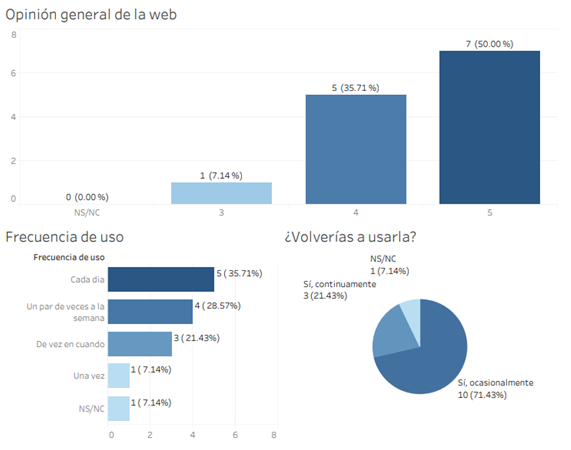
\includegraphics[width=12cm]{enqueteResults}
   \caption{Part of the user experience enquete results}
\end{figure}

Most of the respondents agreed that the functionality they liked the most, was to see the air quality index actually in the
map, and suggested increasing the number of zones.
92 \% of the respondents found the information useful and complete, and 71.43 \% answered that they also found it
understandable.
More than half of the respondents admit that they did not know the meaning of the air quality index, but after
using the tool, they now understand it.
Regarding their interest about air quality, half of them indicated that they had never sought information about it,
only two were previously well informed, and one of them marked the 'other' option and specified that using the application had aroused their interest.
In addition, four of them indicated that, thanks to the tool, they have now discovered they have a medical condition that is affected by air quality.

Among the test subjects, a greater awareness of pollution has been recognized, and they now show more interest in the
air quality in the city and its possible effects on their health.

